\begin{center}
Problema H

Genes Significativos

{\tiny Por Heverton Barros de Macêdo}

Timelimit: $1$	
\end{center}

{\footnotesize
Charles, um famoso pesquisador da evolução das espécies passou a investigar vidas artificiais. Em seus estudos, constatou que para cada amostra genética de um indivíduo da população estudada apenas alguns genes são significativos. A suposição do pesquisador para encontrar os genes significativos é um tanto quanto curiosa e foi realizada da seguinte forma:

Inicialmente foi defino um número para cada gene que pode variar de 0 a 10000. A quantidade de genes para cada indivíduo não é conhecida, mas para fins de estudos foi estipulada como variando de 1 a 100. A partir da sequência genética é montada uma espécie de hierarquia, no formato de um organograma, em que o primeiro gene é o pai. A partir do segundo gene, a inserção no organograma ocorre multiplicando o número do gene pai com o número do gene que está sendo inserido, para então extrair os seus dois últimos dígitos, que definem o chamado valor hierárquico. O valor hierárquico é responsável por indicar a posição no organograma em que esse gene será inserido. Uma restrição na construção do organograma é que cada gene possui 4 filhos, nomeados como filho1, filho2, filho3 e filho4, em que cada filho representa 1/4 do valor hierárquico (filho1 de 0 a 24, filho2 de 25 a 49, filho3 de 50 a 74 e filho4 de 75 a 99).

De posse do organograma, a extração dos genes significativos é obtida conforme o nível em que o gene se encontra, mas não se sabe ao certo em qual nível da hierarquia estão os genes significativos.

Para exemplificar, considere a seguinte sequência genética de um indivíduo: 1023 56 2981 517 2 5 8 479 1052 69

A construção do organograma incia com o primeiro gene 1023 que representa o pai na hierarquia. Em seguida, o gene 56 é multiplicado com o pai (1023) produzindo o número 57288, onde então é obtido o valor hierárquico 88, indicando que o gene 56 será inserido no organograma como filho4 de 1023. Graficamente podemos representar como:

\begin{figure}[ht]
\centering
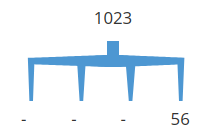
\includegraphics[width=2.5cm]{fig/h_1.png}
\label{Estrutura hierárquica com dois genes}
\end{figure}

Na sequência, o gene 2981, é inserido no organograma de forma similar, primeiro multiplicando com 1023, produzindo o número 3049563, onde se obtém o valor hierárquico 63, o que indica que será inserido como filho3 de 1023. 

\begin{figure}[ht]
\centering
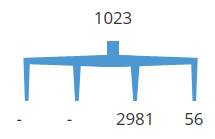
\includegraphics[width=2.5cm]{fig/h_2.png}
\label{Estrutura hierárquica com três genes}
\end{figure}

O terceiro gene, 517, será inserido como filho3 de 56, visto que inicialmente ocorre a multiplicação de 1023 por 517, produzindo o número 528891, onde se obtém o valor hierárquico 91, indicando que este deveria ser inserido como filho4 de 1023, porém, essa posição já está ocupada, e o processo é então repetido, considerando como pai o gene 56. Multiplicando 56 por 517 será produzido o número 28952 que indica o valor hierárquico 52, ocorrendo assim a inserção do gene 517 como filho3 de 56.

Para a sequência genética do exemplo, podemos obter graficamente o organograma abaixo:

\begin{figure}[ht]
\centering
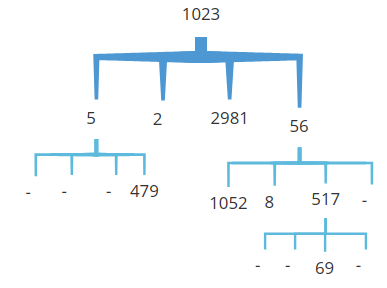
\includegraphics[width=5cm]{fig/h_3.png}
\label{Estrutura hierárquica completa para o exemplo}
\end{figure}

Considerando que os genes significativos do exemplo citado estão no nível 2 do organograma, começando a contagem de níveis em 0, temos como genes significativos: 479, 1052, 8 e 517.

Sua missão é ajudar Charles a obter os genes significativos de um indivíduo e acelerar os estudos desse pesquisador.

\vspace{0.3cm}
\textbf{Entrada}
Cada entrada contém os dados de um indivíduo. A primeira linha contém um inteiro $X$ indicando o nível (iniciado em 0) da hierarquia onde estão os genes $(0 \leq X \leq 99)$. A segunda linha representa a quantidade $N$ de genes de um indivíduo $(1 \leq N \leq 100)$. A terceira linha é formada pela sequência $S$ de genes de um indivíduo, sendo que cada elemento está no intervalo de $0$ a $10000$ $(0 \leq S[i] \leq 10000, 0 \leq i < N)$.

\vspace{0.3cm}
\textbf{Saída}
O sistema deve retornar a sequência de genes significativos seguido do caractere \#, todos separados por um único espaço, conforme o nível hierárquico $X$, indicado na primeira linha da entrada. Os filhos 1, 2, 3 e 4, devem ser representados da esquerda para direta. Se nenhum gene significativo for encontrado no nível indicado, a saída terá apenas o caractere \#.

\begin{table}[h]
    \centering
    \begin{tabular}{|p{8cm}|p{7cm}|}
        \hline
        \begin{center}
            \vspace{-0.3cm}
            \textbf{Exemplos de Entrada}
            \vspace{-0.3cm}
        \end{center} 
         &  
        \begin{center}
            \vspace{-0.3cm}
            \textbf{Exemplos de Saída}
            \vspace{-0.3cm}
        \end{center} \\ \hline
         \texttt{0} & \texttt{1023 \#} \\  
         \texttt{10} & \texttt{} \\  
         \texttt{1023 56 2981 517 2 5 8 479 1052 69} & \texttt{} \\
         \hline
         \texttt{2} & \texttt{479 1052 8 517 \#} \\  
         \texttt{10} & \texttt{} \\  
         \texttt{1023 56 2981 517 2 5 8 479 1052 69} & \texttt{} \\
         \hline    
         \texttt{5} & \texttt{\#} \\  
         \texttt{10} & \texttt{} \\  
         \texttt{1023 56 2981 517 2 5 8 479 1052 69} & \texttt{} \\
         \hline    
         \texttt{2} & \texttt{2501 25 38 78 \#} \\  
         \texttt{10} & \texttt{} \\  
         \texttt{5 98 78 50 7 38 25 61 1579 2501} & \texttt{} \\
         \hline    
    \end{tabular}
    \caption{Exemplos de entradas e saídas}
    \label{tab:inputHProblem}
\end{table}}

\newpage

\begin{center}
\lstinputlisting{abobora_23/H/H3.cpp}
\end{center}
